\documentclass{article}

% if you need to pass options to natbib, use, e.g.:
% \PassOptionsToPackage{numbers, compress}{natbib}
% before loading nips_2016
%
% to avoid loading the natbib package, add option nonatbib:
% \usepackage[nonatbib]{nips_2016}

\usepackage[final]{nips_2016}

% to compile a camera-ready version, add the [final] option, e.g.:
% \usepackage[final]{nips_2016}

\usepackage[utf8]{inputenc} % allow utf-8 input
\usepackage[T1]{fontenc}    % use 8-bit T1 fonts
\usepackage{hyperref}       % hyperlinks
\usepackage{url}            % simple URL typesetting
\usepackage{booktabs}       % professional-quality tables
\usepackage{amsfonts}       % blackboard math symbols
%\usepackage{nicefrac}       % compact symbols for 1/2, etc.
\usepackage{microtype}      % microtypography

\usepackage{amssymb, amsmath}
\usepackage{epsfig}
\usepackage{array}
\usepackage{ifthen}
\usepackage{color}
\usepackage{fancyhdr}
\usepackage{graphicx}
\usepackage{mathtools}
\usepackage{csquotes}

\newcommand{\tr}{\text{tr}}
\newcommand{\E}{\textbf{E}}
\newcommand{\diag}{\text{diag}}
\newcommand{\argmax}{\text{argmax}}
\newcommand{\Cov}{\text{Cov}}
\newcommand{\Var}{\text{Var}}
\newcommand{\argmin}{\text{argmin}}
\newcommand{\Vol}{\text{Vol}}
\newcommand{\comm}[1]{}
\newcommand{\indep}{\rotatebox[origin=c]{90}{$\models$}}
\newcommand{\Cor}{\text{Cor}}

\title{Estimating mutual information in high dimensions via classification error}

% The \author macro works with any number of authors. There are two
% commands used to separate the names and addresses of multiple
% authors: \And and \AND.
%
% Using \And between authors leaves it to LaTeX to determine where to
% break the lines. Using \AND forces a line break at that point. So,
% if LaTeX puts 3 of 4 authors names on the first line, and the last
% on the second line, try using \AND instead of \And before the third
% author name.

\author{
  Charles Y.~Zheng \\
  Department of Statistics\\
  Stanford University\\
  Stanford, CA 94305 \\
  \texttt{snarles@stanford.edu} \\
  %% examples of more authors
  \And
  Yuval ~Benjamini \\
  Department of Statistics \\
  Hebrew University\\
  Jerusalem, Israel\\
  \texttt{yuval.benjamini@mail.huji.ac.il}
  %% Address \\
  %% \texttt{email} \\
  %% \AND
  %% Coauthor \\
  %% Affiliation \\
  %% Address \\
  %% \texttt{email} \\
  %% \And
  %% Coauthor \\
  %% Affiliation \\
  %% Address \\
  %% \texttt{email} \\
  %% \And
  %% Coauthor \\
  %% Affiliation \\
  %% Address \\
  %% \texttt{email} \\
}

\begin{document}
% \nipsfinalcopy is no longer used

\maketitle

\begin{abstract}
Estimating the mutual information $I(X; Y)$ based on observations
becomes statistically infeasible in high dimensions without some kind
of assumption or prior.  One approach is to assume a parametric joint
distribution on $(X, Y)$, but in many applications, such a strong
modeling assumption cannot be justified.  Alternatively, one can estimate the mutual information based the performance of a classifier trained on the data.  Existing methods include using the empirical mutual information of the confusion matrix of the classifier, as
well as an estimator based on Fano's inequality.  However, both of these
methods all produce an estimate which is bounded by $\log(k)$,
where $k$ is the number of classes.
This presents a substantial limitation for classification-based approaches, since the number of
repeats per class must be large for the classifier to work well, hence limiting the number of classes $k$ that can be defined. In this paper, we construct a novel classification-based estimator of mutual information which
overcomes these limitations.  Our estimator is based on
high-dimensional asymptotics: we show that in a particular limiting
regime, the mutual information is an invertible function of the
expected $k$-class Bayes error.  While the theory is based
on a large-sample, high-dimensional limit, we demonstrate through
simulations that our proposed lower confidence bound has superior
performance to the alternatives in problems of moderate
dimensionality.
\end{abstract}

\section{Introduction}

Mutual information $I(X; Y)$ is fundamentally a measure of dependence
between random variables $X$ and $Y$, and is defined as
\[
I(X;Y) = \int p(x, y) \log \frac{p(x, y)}{p(x)p(y)}dxdy.
\]
In its original context of information theory, the mutual information
describes the rate at which a noisy communications channel $Y$ can
communicate bits from a source stream $X$, but by now, the quantity
$I(X, Y)$ has found many new uses in science and engineering.  Mutual
information is used to test for conditional independence (CITE), to
quantifying the information between a random stimulus $X$ and the
signaling behavior of an ensembles of neurons, $Y$ (Borst 1999); for
use as an objective function for training neural networks (CITE), for
feature selection in machine learning, and even as an all-purpose
nonlinear measure of ``correlation for the 21st century'' (Speed.)
What is common to all of these new applications, and what differs from
the original setting of Shannon's theory of information, is that the
variables $X$ and $Y$ have unknown distributions which must be
inferred from data.  In the case when $X$ and $Y$ are both
low-dimensional, for instance, when summarizing the properties of a
single neuron in response to a single stimulus feature, $I(X; Y)$ can
be estimated nonparametrically using a reasonable number of
observations.  There exists a huge literature on nonparametric
estimation of entropy and mutual information exists, see (CITE) for a
review.

However, the sample complexity for nonparametric estimation grows
exponentially with the dimension, rendering such methods ineffective
in applications with high-dimensional data.  One such application
includes multivariate pattern analysis (MVPA), an area of neuroscience
research pioneered by Haxby (2001), which studies how entire regions
of the human brain respond to stimuli, using function magnetic
resonance imaging (fMRI) data; in MVPA studies, the input $X$ could be
a natural image parameterized by $p = 10000$ image features, while the
output $Y$ is a $q=20000$-dimensional vector of brain activation
features obtained from the fMRI scan.  In problems of such
dimensionality, one can tractably estimate mutual information by
assuming a multivariate Gaussian model: however, this approach
essentially assumes a linear relationship between the input and
output, and hence fails to quantify nonlinear dependencies.  Rather
than assuming a full parametric generative model, one can empirically
select a good \emph{discriminative} model by using machine learning.
Treves (1997) first proposed using the empirical mutual information of
the classification matrix in order to obtain a lower bound of the
mutual information $I(X; Y)$; this confusion-matrix-based lower bound
has subsequently enjoyed widespread use in the MVPA literature
(Quiroga 2009.)  But even earlier that this, the idea of linking
classification performance to mutual information can be found in the
beginnings of information theory: after all, Shannon's original
motivation was to characterize the minimum achievable error
probability of a noisy communication channel.  More explicitly, Fano's
inequality provides a lower bound on mutual information in relation to
the optimal prediction error, or Bayes error. 

The estimator based on the confusion matrix, $\hat{I}_{CM}$, and
the estimator based on Fano's inequality, $\hat{I}_{Fano}$, are two examples of what
might be called the \emph{discriminative} approach to mutual
information estimation, in contrast to the \emph{parametric} and
\emph{nonparametric} approaches.  In many applications, the
discriminative approach takes an advantageous middle ground between
the two extremes of nonparametric and parametric approaches for
estimating mutual information. In neuroimaging data, we lack prior
knowledge for specifying parametric models, and the data is too
high-dimensional for nonparametric approaches, but we have a
sufficient idea of the general ``structure'' in the data to achieve
above-chance classification rates.

But as noted in the literature (Quiroga et al. 2009), such
discriminative approaches generally underestmate the mutual information.  Two sources of
``information loss'' are (1) the fact that a continuous input variable
$X$ is discretized into $k$ classes, and (2) that the performance of
any classifier trained from data can at best given an \emph{upper
  bound} to the error of the best classification rule: the Bayes
error. Furthermore, all existing discriminative estimators of mutual information share the
limitation that $\hat{I}$ is a \emph{bounded} estimator:
$\hat{I} \in [0, \log(k)]$
where $k$ is the number of classes defined in the classification task.
This is a reasonable limitation, since one can construct a worst-case
example where the $I(X; Y) = \log(k)$ and the Bayes error has a
positive probability of equalling zero\footnote{Let $p(x, y) =
  I(\min(|x - y|, |x - y + 1|) < \frac{1}{k})$ over the unit square,
  and assume that stratified sampling is used to define the classes
  (see section 1.1).}.  However, in situations where we can rule out
such pathological cases, an \emph{unbounded} estimate of mutual
information could potentially outperform $\hat{I}_{Fano}$ and
$\hat{I}_{CM}$, especially if $I(X; Y) \gg \log(k)$.

What we propose in this paper is to exploit an assumption of
\emph{high dimensionality} in order to rule out pathological cases
where the mutual information becomes decoupled from the classification
error.  This assumption of high dimensionality is well-suited for the
applications where discriminative approaches for estimating mutual
information are appropriate.  In section 2 we present an asymptotic
setting intended to capture the notion of high dimensionality; namely,
one where the number of classes is fixed, and where the information
$I(X; Y)$ remains fixed, while the dimensionality of the input $X$ and
output $Y$ both grow to infinity.  We make a number of additional
regularity conditions to rule out scenarios where $(X, Y)$ is really
less ``high-dimensional'' than it appears, since most of the variation
is captured a low-dimensional manifold.  In section 2.2 we present our
key result, which links the asymptotic average Bayes error to the
mutual information; in section 2.3 we apply this result to derive our
proposed estimator, $\hat{I}_{HD}$ (where HD stands for ``high-dimensional.'')  Section 3 presents
simulation results, and section 4 concludes.  All proofs are given in the supplemental material for space reasons.

\subsection{Discriminative estimators of mutual information}

Before presenting our asymptotic analysis, we provide some background
on discriminative methods for estimating mutual information and
define the sampling assumptions behind our procedure.

Assume that the variables $X, Y$ have a joint distribution $F$, and
that one can define a conditional distribution of $Y$ given $X$,
$Y|X \sim F_X,$
and let $G$ denote the marginal distribution of $X$.
We consider two different types of sampling procedures:
\begin{itemize}
\item \emph{pair sampling}:  For $i = 1,\hdots, n$, the data $(X^i, Y^i)$ are sampled i.i.d. from the joint distribution of $(X, Y)$.
\item \emph{stratified sampling}:  For $j = 1,\hdots, k$, sample i.i.d. \emph{exemplars} $X^{(1)},\hdots, X^{(k)} \sim G$.  For $i = 1,\hdots, n$, draw $Z^i$ iid from the uniform distribution on $1,\hdots, k$, then draw $Y^i$ from the conditional distribution $F_{X^{(Z_i)}}$.
\end{itemize}

Pair sampling occurs in observational studies, where one observes both $X$ and $Y$ externally.  On the other hand, stratified sampling is more commonly seen in controlled experiments, where an experimenter chooses an input $X$ to feed into a black box, which outputs $Y$.  An example from fMRI studies is an experimental design where the subject is presented a stimulus $X$, and the experimenter measures the subject's response via the brain activation $Y$. \footnote{Note the asymmetry in our definition of stratified sampling: our convention is to take $X$ to be the variable preceding $Y$ in causal order.  Such causal directionality constrains the stratified sampling to have repeated $X$ rather than repeated $Y$ values, but has no consequence for the mutual information $I(X; Y)$, which is a symmetric function.}

Given data from either pair sampling or stratified sampling, one can define various
\emph{classification tasks}.  Here, the point is to use classification as a tool for extracting information
about the relationship between $X$ and $Y$.  As such, it is up to us to define the classification tasks
of interest.  For instance, one can define tasks which either classify $Y$ based on $X$, or classify $X$ based on $Y$; without loss of generality, we henceforth consider the latter.  In the case of continuous $X$, we can define an arbitrary number of classes $k$ by specifying a partition on the space of $X$.
That is, one can define a \emph{class function} $Z: X \to \{1,\hdots, k\}$, and consider the problem of classifying $Z$ given $Y$.  A classification rule is
any (possibly stochastic) mapping $f: \mathcal{Y} \to \{1,\hdots,
k\}$, where $\mathcal{Y}$ is a superset of the support of $Y$.  The \emph{generalization error} of the classification rule is
$
e_{gen}(f) = Pr[f(Y) \neq Z].
$
The Bayes error is the generalization error of the optimal classification rule,
$
e_{Bayes}(f) = \inf_f e_{gen}(f)
$
We call such a classification task a \emph{partition-based} classification task.

The freedom to choose the partition $Z$ may be more of a curse than a blessing when it is unclear how
to choose an appropriate partition on the support of $X$.  If stratified sampling is employed,
one can define an \emph{exemplar-based} classification task which avoids having to specify a partition.  One defines the \emph{class function} $Z$ by
\[
Z: \{X^{(1)}, \hdots, X^{(k)}\} \to \{1,\hdots, k\},
\]
\[
Z(X^{(i)}) = i\text{ for }i = 1, \hdots, k.
\]
Note that the domain of $Z$ is restricted to the set of observed exemplars $X^{(1)},\hdots, X^{(k)}$.
The loss function is not well-defined when $X$ lies outside the set of exemplars,
so it is natural to define the generalization error by
\[
e_{gen}(f) = \frac{1}{k} \sum_{i=1}^k\Pr[f(Y) \neq Z|X = X^{(i)}].
\]
Indeed, in experiments where stratified sampling is used, this is the most commonly employed notion
of generalization error (CITE).

In an exemplar-based classification, there is no need to specify an arbitrary partition on the input space, but now the $k$ classes will now be \emph{randomly} defined.  One consequence is that the Bayes error $e_{Bayes}$ is a random variable: when the sampling produces $k$ similar exemplars, $e_{Bayes}$ will be higher, and when the sampling produces well-separated exemplars $e_{Bayes}$ may be lower.  
Therefore it is useful to consider the \emph{average Bayes error},
\[
e_{ABE, k} = \E_{X^{(1)},\hdots, X^{(k)}}[e_{Bayes}]
\]
where the expectation is taken over the joint distribution of $X^{(1)},\hdots, X^{(k)} \stackrel{iid}{\sim} G$.

While partition-based classification tasks are the most commonly encountered classification tasks
in the scientific and engineering literature, for the current paper we choose to focus on
exemplar-based classification tasks.  The reason we focus on the exemplar-based setting
is due to mathematical convenience: it is much harder to link population parameters of $(X, Y)$
to the classification task when the classes are defined in a restricted rather than fully arbitrary manner.
Furthermore, for the sake of notational convenience, assume that the sampling
is evenly divided between the classes, with $r$ observations of the output $Y^{(i),1},\hdots, Y^{(1), r}$
for each exemplar $X^{(1)}$.


We have not yet specified how any classification rule $f$ is to be
obtained.  Unless expert knowledge is available, it is usually necessary to choose the function $f$ in a
data-dependent way in order to obtain a reasonable classification
rule.  A wide variety of machine learning algorithms exist for
``learning'' good classification rules $f$ from data.  We use the
terminology \emph{classifier} to refer to any algorithm which takes
data as input, and produces a classification rule $f$ as output.  The
following discussion makes it necessary for us to make a precise
distinction between the \emph{classifier} and the \emph{classification
rule} it produces, and our usage of the terms may differ from the
standard in the literature.  Mathematically speaking, the classifier
is a functional which maps a set of observations to a classification
rule,
\[
\mathcal{F}: \{(x^{1},y^{1}),\hdots, (x^{m}, y^{m})\} \mapsto f(\cdot).
\]
The data $(x^1,y^1),\hdots, (x^m, y^m)$ used to obtain the
classification rule is called \emph{training data.}  When the
objective is to obtain the best possible classification rule, as is
the case in diagnostic settings, it is optimal to use all of the
availible data to train the classifier.  However, when the goal is to
obtain \emph{inference} about the generalization error $e_{gen}$ of the classification
rule $f$, it becomes necessary to split the data into two independent sets:
one set to train the classifier, and one to evaluate the performance.
The reason that such a splitting is necessary is because using the
same data to test and train a classifier introduces significant bias
into the empirical classification error.

In \emph{data-splitting}, one creates a \emph{training
set} consisting of $r_1$ repeats per class,
$
S_{train} = \{(x^{(i)}, y^{(i),j})\}_{i=1, j=1}^{k, r_1},
$
and a \emph{test set} consisting of the remaining $r_2 = r - r_1$ repeats,
$
S_{test} = \{(x^{(i)}, y^{(i),j})\}_{i=1, j=r_1}^{k, r}.
$
One inputs the training data into the classifier to obtain the classification rule
$
f = \mathcal{F}(S_{train}).
$
The performance of the classifier is evaluated by predicting the classes of the test set.
The results of this test are summarized by a $k \times k$ \emph{confusion matrix} $M$ with
$
M_{ij} = \sum_{\ell=r_1 + 1}^r I(f(y^{(i), r}) = j).
$
The $i, j$th entry of $M$ counts how many times a output in the $i$th class was classified  to the $j$th class.
The \emph{test error} is the proportion of off-diagonal terms of $M$,
$
e_{test} = \frac{1}{kr} \sum_{i \neq j} M_{ij},
$
and is an unbiased estimator of $e_{gen}$.
However, in small sampling regimes the quantity $e_{test}$ may be too variable to use as an estimator of $e_{gen}$.  We recommend the use of Bayesian smoothing, defining an  $\alpha$-smoothed estimate $\hat{e}_{gen, \alpha}$ by
$
\hat{e}_{gen, \alpha} = (1 - \alpha) e_{test} + \alpha \frac{k-1}{k},
$
which takes a weighted average of the unbiased estimate $e_{test}$, and the natural prior of \emph{chance classification}.

We are now ready to define the family of \emph{discriminative estimators} of mutual information.
A discriminative estimator takes the form of a function which maps the misclassification matrix to a positive number,
$
\hat{I}: \mathbb{N}^{k \times k} \to \mathbb{R}.
$
We are aware of the following examples of discriminative estimators: (1) estimators derived from using Fano's inequality, and (2) the empirical information of the confusion matrix, as introduced by Treves (1999).

Fano's inequality can be easily adapted to yield a discriminative estimator.
The original inequality reads
\[
H(Z|Y) \leq H(e_{Bayes}) + e_{Bayes} \log ||\mathcal{Z}| - 1|
\]
where $H(e)$ is the entropy of a Bernoulli random variable with probability $e$.
Replacing $H(Z|Y)$ with $H(X|Y)$ and replacing $e_{Bayes}$ with $\hat{e}_{gen, \alpha}$,
we get the estimator
\[
\hat{I}_{Fano}(M) = log(K) - \hat{e}_{gen, \alpha} log(K-1) + \hat{e}_{gen, \alpha} log(p) + (1-\hat{e}_{gen, \alpha}) log(1-\hat{e}_{gen, \alpha}).
\]
Supposing that $H(Z|Y) \leq H(X|Y)$ and $\hat{e}_{gen, \alpha} \leq e_{Bayes}$, we have
\[\hat{I}_{Fano} \leq I(X; Y).\]
In the partition-based classification task, $Z$ can be defined to be uniformly distributed, which ensures that  $H(Z|Y) \leq H(X|Y)$.  Hence, replacing $\hat{e}_{gen,\alpha}$ with an upper confidence bound, one can produce a lower confidence bound for $I(X; Y)$ using Fano's inequality.
However, in the stratified regime, one cannot bound the probabilities of the event $H(Z|Y) > H(X|Y)$,
so $\hat{I}_{Fano}$ cannot be easily adapted into a lower confidence bound.

The confusion matrix approach computes
\[
\hat{I}_{CM}(M) = \frac{1}{k^2} \sum_{i=1}^k \sum_{j=1}^k \log \frac{M_{ij}}{r/k},
\]
which is the empirical mutual information of the discrete joint distribution $(Z, f(Y))$.

It is easy to show that $\log(k)$ is a tight upper bound for both estimators.
Tightness is achieved in a discrete example where $Y = Z$, and $Z$ is uniform on $\{1,\hdots, k\}$.
The fact that $\log(k)$ upper bounds the estimator $\hat{I}$ substantially limits the estimator's usefulness when $I(X; Y)$ is large.  As $I(X; Y)$ exceeds $\log(k)$, the estimate $\hat{I}$ can no longer approximate $I(X; Y)$ even up to a constant factor.

The \emph{undersampled} regime, where $k \ll e^{I(X; Y)}$ is also problematic for nonparametric estimators of mutual information.
Gastpar et al. (2009), studied the nonparametric estimator
\[
\hat{I}_0 = \hat{H}(Y) - \frac{1}{k}\sum_{i=1}\hat{H}(Y|X),
\]
where $\hat{H}$ is an estimator for the entropy.
Gastpar et al. showed that $\hat{I}_0$ is biased downwards due to undersampling of the exemplars:
to counteract this bias, they introduce the anthropic correction estimator $\hat{I}_\alpha$.\footnote{
If the parameter $\alpha \in [0, 1)$ is chosen correctly, the estimator is unbiased, but no method is given to tune the parameter.  Gastpar also suggest using $[\hat{I}_0, \hat{I}_1]$ as an interval estimate of the mutual information, but in many high-dimensional cases $\hat{I}_1$ can be infinite.
}

Meanwhile, the parametric approach is relatively robust to undersampling of the exemplars.
For instance, in the multivariate Gaussian model, the mutual information is a function of the eigenvalues of the canonical correlation matrix $R  =\Sigma_X^{-1/2}\Sigma_{XY}\Sigma_Y^{-1/2}$.  If $X$ is a controlled stimulus, $\Sigma_X$ can be taken to be identity, and the interclass covariance matrix of $Y$ suffices to estimate $\Sigma_Y$ consistently.  The remaining parameter $\Sigma_{XY}$ can be estimated from the inner-product matrix $\boldsymbol{X}^T \boldsymbol{Y}$, which is unbiased for $\Sigma_{XY}$ regardless of whether pair sampling or stratified sampling is employed.

Therefore a possible approach to overcoming the $\log(k)$ barrier in a discriminative estimator
is to make stronger assumptions on the distributional properties of $Y|X$.  Assuming a fully specified
parametric model defeats the purpose of the discriminative approach.  But one remaining hope is
to appeal to a \emph{unversality principle}, such as central limit theorem. Perhaps regularity can be achieved
without making overly strong assumptions, if a principle such as CLT ensures that a wide variety of
distributions all share similar behavior in some limit.  This is the basis of our high-dimensional
approach to discriminative estimation of mutual information, where the assumption of high dimensionality,
combined with application of the central limit theorem, provides the needed universality.

\section{Theory}

As we already emphasized in the introduction, we can derive a new discriminative estimator 
by considering a high-dimensional regime, which we fully detail in section 2.1.
The key benefit of this high-dimensional regime, is that it allows us to establish a relationship between the
mutual information $I(X; Y)$ and the $k$-class average Bayes error,
$e_{ABE, k}$.  In short, we will identify a function $\pi_k$
(which depends on $k$),
\[
e_{ABE, k} \approx \pi_k(\sqrt{2 I(X; Y)})
\]
and that this approximation becomes accurate under a limit where $I(X; Y)$ is small relative to the dimensionality of $X$,
and under the condition that the components of $X$ are approximately independent.
The function $\pi_k$ is given by
\[
\pi_k(c) = 1 - \int_{\mathbb{R}} \phi(z - c)  \Phi(z)^{k-1} dz.
\]
%One way of intuitively understanding $1-\pi_k$ is that a misclassification event is when one of the...
Figure \ref{fig:pi} displays the plot of $\pi_k$ for several values of $k$.
For all values of $k$, $\pi_k(\mu)$ is monotonically decreasing in $\mu$, and tends to zero as $\mu \to \infty$.
This should not be surprising, because if $I(X; Y)$ is large, then the average Bayes error should be small.
Another fact, which can be verified through a simple calculation, is that 
$
\pi_k(0) = 1 - \frac{1}{k}.
$
This should also not be surprising, since if $I(X; Y) = 0$, then it should not be possible to
obtain a classification rule which is better than guessing at random, which is only correct with probability $1/k$.
\begin{figure}
\centering
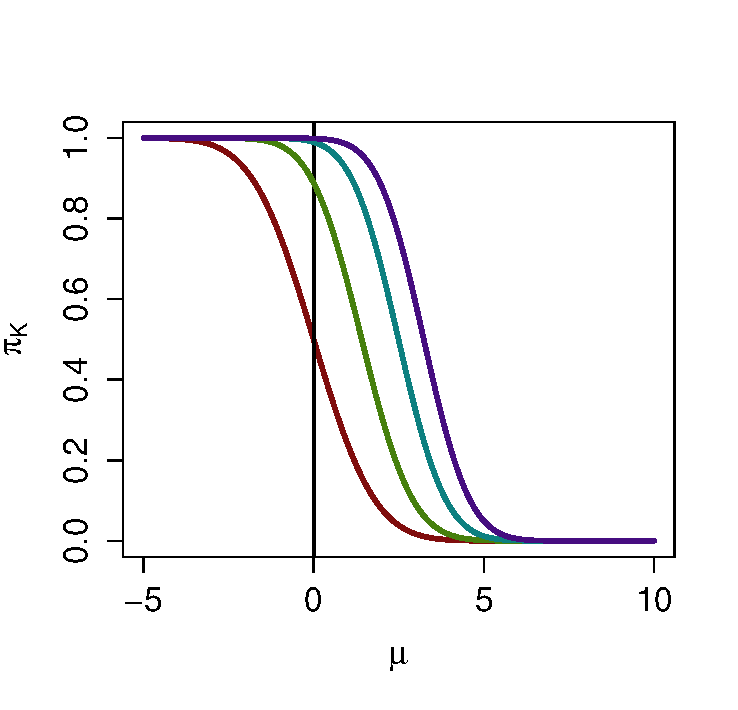
\includegraphics[scale = 0.5, clip=true, trim=0 0.2in 0 0.5in]{../info_theory_sims/illus_piK.pdf}
\caption{The function $pi_k(\mu)$, for $k = \{2, 9, 99, 999\}$ (left to right) \label{fig:pi}}
\end{figure}

First, we rewrite the average Bayes error as
\begin{align}
e_{ABE, k} &= \frac{1}{k}\sum_{i=1}^k \E[\Pr[p(Y|x_i) \leq \max_{j \neq i} p(Y|x_j)| X = x_i]]
\\&= \E[\Pr[p(Y|x_1) \leq \max_{j \neq 1} p(Y|x_j)| X = x_1]]
\\&= \Pr[p(Y|X_1) \leq \max_{j \neq 1} p(Y|X_j)| X = X_1].
\end{align}

Defining $Z_i = \log p(Y|X_i) - \log p(Y|X_1)$, where $Y \sim p(y|X_1)$.
The we obtain
\[
e_{ABE} = \Pr[Z_1 < \max_{j > 1} Z_i].
\]

Our proof uses the assumption that $Z_1,\hdots, Z_k$ are asymptotically multivariate normal.
Supposing that $Z_1,\hdots, Z_k$ are indeed asymptotically normal, the following lemma
allows us to obtain a formula for the misclassification rate.

\textbf{Lemma 1. }
\emph{
Suppose $(Z_1, Z_2, \hdots, Z_k)$ are jointly multivariate normal, with 
$\E[Z_1 - Z_i]= \alpha$, 
$\Var(Z_1) = \beta$, 
$\Cov(Z_1, Z_i) = \gamma$, 
$\Var(Z_i)= \delta$, and $\Cov(Z_i, Z_j) = \epsilon$ for all $i, j = 2, \hdots,
k$, such that $\beta + \epsilon - 2\gamma > 0$.  Then, letting
\[
\mu = \frac{\E[Z_1 - Z_i]}{\sqrt{\frac{1}{2}\Var(Z_i - Z_j)}} = \frac{\alpha}{\sqrt{\delta - \epsilon}},
\]
\[
\nu^2 = \frac{\Cov(Z_1 -Z_i, Z_1 - Z_j)}{\frac{1}{2}\Var(Z_i - Z_j)} = \frac{\beta + \epsilon - 2\gamma}{\delta - \epsilon},
\]
we have
\begin{align*}
\Pr[Z_1 < \max_{i=2}^k Z_i] &= \Pr[W < M_{k-1}]
\\&= 1 - \int \frac{1}{\sqrt{2\pi\nu^2}} e^{-\frac{(w-\mu)^2}{2\nu^2}} \Phi(w)^{k-1} dw,
\end{align*}
where $W \sim N(\mu, \nu^2)$ and $M_{k-1}$ is the maximum of $k-1$
independent standard normal variates, which are independent of $W$.
}

To see why the assumption that $Z_1,\hdots, Z_k$ are multivariate normal might be justified, suppose that $X$ and $Y$ have the same dimensionality $d$, and that
joint density factorizes as
\[
p(x_j, y) = \prod_{i=1}^d p_i(x_{j, i}, y_i)
\]
where $x_{j, i}, y_i$ are the components of $x_j$ and $y$.
Then,
\[
Z_i = \sum_{m=1}^d \log p_m(y_m | x_{m, i}) - \log p_m(y_m | x_{m, 1})
\]
where $x_{i, j}$ is the $i$th component of $x_j$.
The $d$ terms $\log p_m(y_m | x_{m, i}) - \log p_m(y_m | x_{m, 1})$ are independent across the indices $m$,
but dependent between the $i = 1,\hdots, k$.
Therefore, the multivariate central limit theorem can be applied to conclude that the vector
$(Z_1,\hdots, Z_k)$ can be scaled to converge to a multivariate normal distribution.
Now, since the average Bayes error $e_{ABE,k}$ is a continuous functional of the joint distribution $p(x, y)$,
it follows that $e_{ABE,k}$ converges to a functional of the limiting mean and covariance of $(Z_1,\hdots, Z_k)$, assuming
that the limits exist.
In our theorem, we assume a specific regime where these limits exist as a consequence.
While the componentwise independence condition is not a realistic assumption,
the key property of multivariate normality of $(Z_1,\hdots, Z_k)$ holds under more general conditions, and appears reasonable in practice.

The second component of our theorem is to manipulate the expression of the mutual information $I(X; Y)$.
The differential mutual information is defined as
\[
I(X; Y) = \int p(x, y) \log \frac{p(x, y)}{p(x) p(y)} dx dy.
\]
The key manipulation we employ is to approximate the logarithmic term by the Taylor expansion
\[
\log \frac{p(x, y)}{p(x) p(y)} \approx \frac{p(x, y) - p(x) p(y)}{p(x) p(y)} - \left(\frac{p(x, y) - p(x) p(y)}{p(x) p(y)}\right)^2 + \hdots.
\]
The approximation is accurate if $I(X; Y)$ is small--or rather, small relative to the dimensionality within the asymptotic sequence.
We state the theorem for the regime where $I(X; Y)$ is fixed, while the dimensionality of $X$ increases.

\textbf{Theorem 1.} Let $p^{[d]}(x, y)$ be a sequence of joint densities
for $d = 1,2,\hdots$ as given above.  Further assume that
\begin{itemize}
\item[A1.] $\lim_{d \to \infty} I(X^{[d]}; Y^{[d]}) = \iota < \infty.$
\item[A2.] There exists a sequence of scaling constants $a_{ij}^{[d]}$
and $b_{ij}^{[d]}$ such that the random vector $(a_{ij}\ell_{ij}^{[d]} +
b_{ij}^{[d]})_{i, j = 1,\hdots, k}$ converges in distribution to a
multivariate normal distribution.
\item[A3.] There exists a sequence of scaling constants $a^{[d]}$, $b^{[d]}$ such that
\[
a^{[d]}u(X^{(1)}, Y^{(2)}) + b^{[d]}
\]
converges in distribution to a univariate normal distribution.
\item[A4.] For all $i \neq k$,
\[\lim_{d \to \infty}\Cov[u(X^{(i)}, Y^{(j)}), u(X^{(k)}, Y^{(j)})] = 0.\]
\end{itemize}
Then for $e_{ABE, k}$ as defined above, we have
\[
\lim_{d \to \infty} e_{ABE, k} = \pi_k(\sqrt{2 \iota})
\]
where
\[
\pi_k(c) = 1 - \int_{\mathbb{R}} \phi(z - c)  \Phi(z)^{k-1} dz
\]
where $\phi$ and $\Phi$ are the standard normal density function and
cumulative distribution function, respectively.

Assumptions A1-A4 are satisfied in a variety of natural models.
One example is a multivariate Gaussian sequence model where
$X \sim N(0, \Sigma_d)$
and 
$
Y = X + E
$ with
$
E \sim N(0, \Sigma_e),
$
where $\Sigma_d$ and $\Sigma_e$ are $d \times d$ covariance matrices, and where $X$ and $E$ are independent.  Then, if $d \Sigma_d$ and $\Sigma_e$ have limiting spectra $H$ and $G$ respectively,
the joint densities $p(x, y)$ for $d = 1,\hdots, $ satisfy assumptions A1 - A4.
Another example is the multvariate logistic model, which we describe in section 3.


\section{Results}

given by
\[
X \sim N(0, I)
\]
\[
Y_i \sim \text{Bernoulli}(e^{\beta X_i}/(1 + e^{\beta X_i}))
\]
The multivariate logistic regression model (and multivariate Poisson regression model)
are especially suitable for modeling neural spike count data;
we simulate data from such a multivariate logistic regression model in section X.


Multiple-response logistic regression model
\[
X \sim N(0, I_p)
\]
\[
Y \in \{0,1\}^q
\]
\[
Y_i|X = x \sim \text{Bernoulli}(x^T B_i)
\]
where $B$ is a $p \times q$ matrix.

\emph{Methods.}
\begin{itemize}
\item \text{Nonparametric}: $\hat{I}_0$ naive estimator, $\hat{I}_\alpha$ anthropic correction.
\item \text{ML-based}: $\hat{I}_{CM}$ confusion matrix, $\hat{I}_F$ Fano, $\hat{I}_{LS}$ low-SNR method.
\end{itemize}

Sampling distribution of $\hat{I}$ for \small{$\{p = 3$, $B = \frac{4}{\sqrt{3}} I_3$, $K = 20$, $r = 40\}$.}

True parameter $I(X; Y) = 0.800$ \emph{(dotted line.)}
\begin{center}
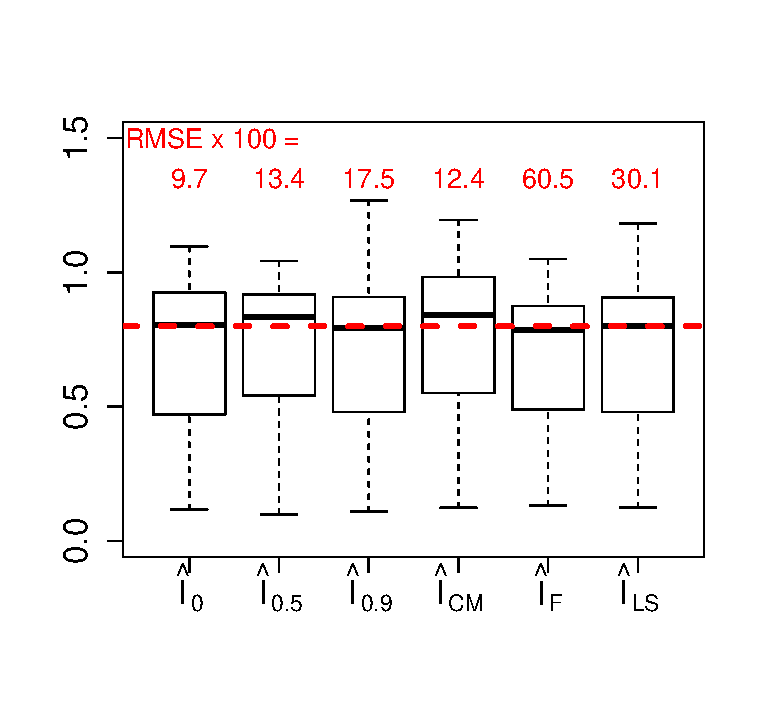
\includegraphics[scale = 0.5, clip = true, trim = 0 0.5in 0 0.5in]{../info_theory_sims/fig1.pdf}
\end{center}
Na\"{i}ve estimator performs best!  $\hat{I}_{LS}$ not effective.

Sampling distribution of $\hat{I}$ for \small{$\{p = 50$, $B = \frac{4}{\sqrt{50}} I_{50}$, $K = 20$, $r = 8000\}$.}

True parameter $I(X; Y) = 1.794$ \emph{(dashed line.)}
\begin{center}
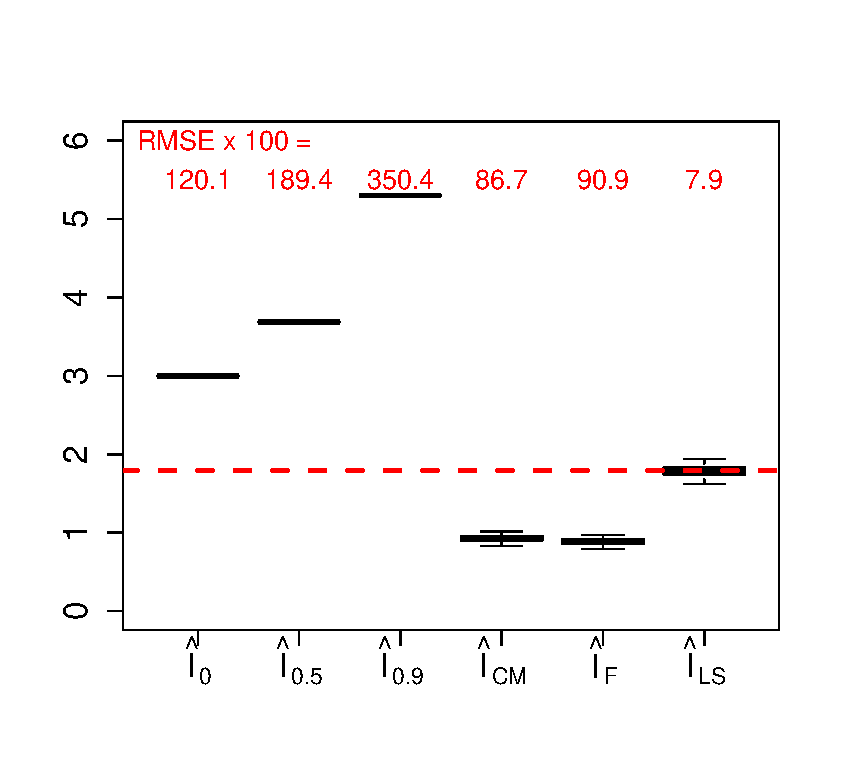
\includegraphics[scale = 0.5, clip = true, trim = 0 0.5in 0 0.5in]{../info_theory_sims/fig2.pdf}
\end{center}
Non-parametric methods extremely biased.

Estimation path of $\hat{I}_{LS}$ and $\hat{I}_\alpha$ as $n$ ranges from $10$ to $8000$.

\small{$\{p = 10$, $B = \frac{4}{\sqrt{10}} I_{10}$, $K = 20\}$.
True parameter $I(X; Y) = 1.322$ \emph{(dashed line.)}}

\begin{center}
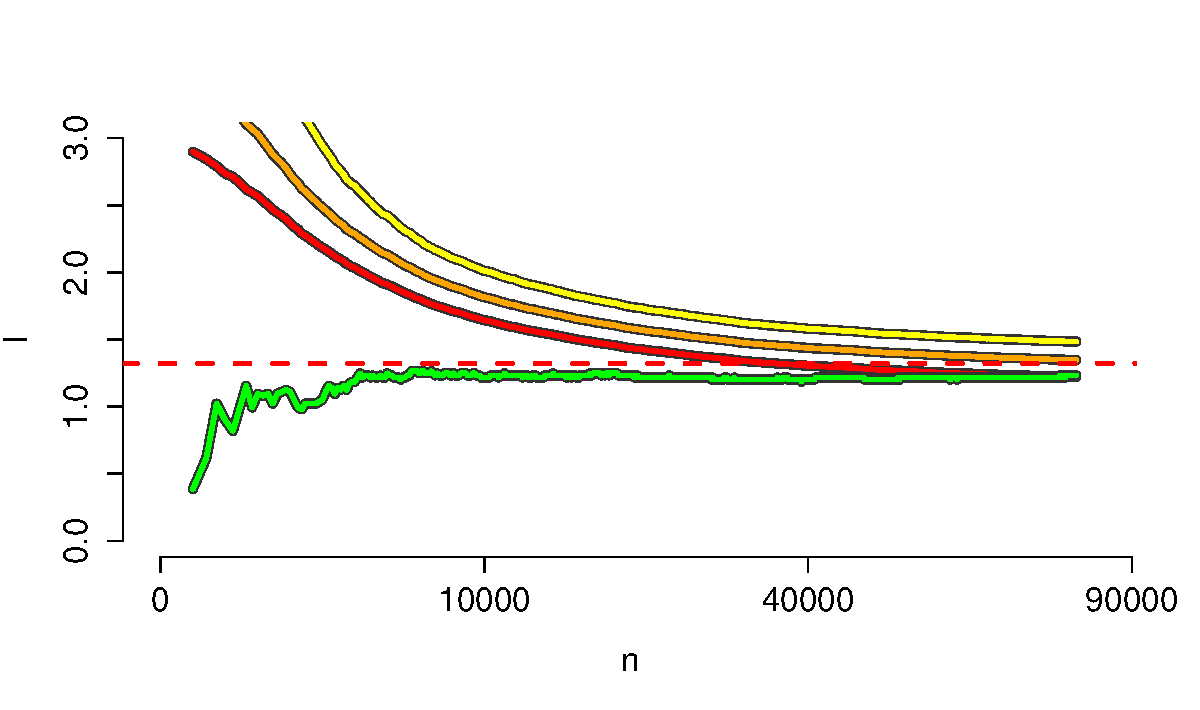
\includegraphics[scale = 0.4]{../info_theory_sims/fig3.pdf}
\end{center}

\begin{center}
\textbf{Estimated $\hat{I}$ vs true $I$.} 

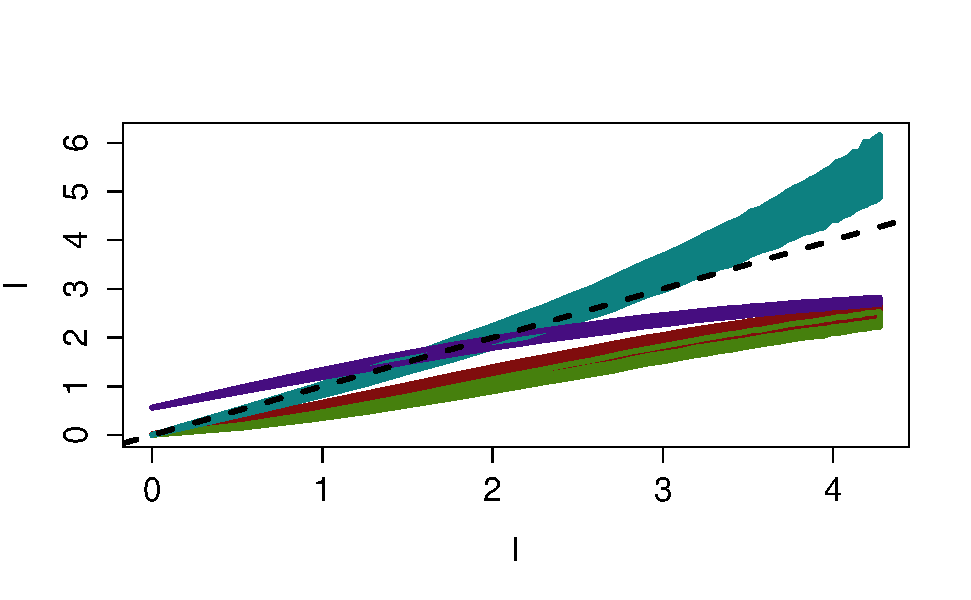
\includegraphics[scale = 0.5, clip=true, trim=0.4in 0.5in 0 0.5in]{../info_theory_sims/fig4.pdf}
\end{center}

Sampling distribution of $\hat{I}_{LS}$ for \small{$\{p = 10$, $B = \frac{4}{\sqrt{10}} I_{10}$, $N = 80000\}$,

and $K = \{5, 10, 15, 20, \hdots, 80\}$, $r = N/k$.}

True parameter $I(X; Y) = 1.322$ \emph{(dashed line.)}
\begin{center}
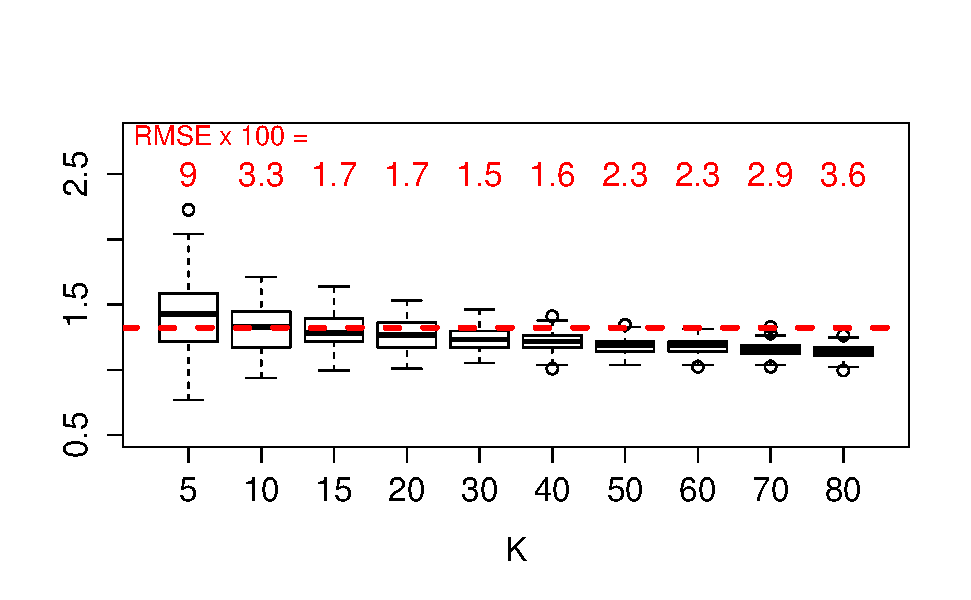
\includegraphics[scale = 0.6, clip = true, trim = 0 0.5in 0 0.5in]{../info_theory_sims/fig5a.pdf}
\end{center}

Decreasing variance as $K$ increases. Bias at large and small $K$.

$p = 20$ and $q = 40$, entries of $B$ are iid $N(0, 0.025)$.

$K=20$, $r = 8000$, true $I(X; Y) = 1.86$ \emph{(dashed line.)}

\begin{center}
\textbf{Sampling distribution of $\hat{I}$.}
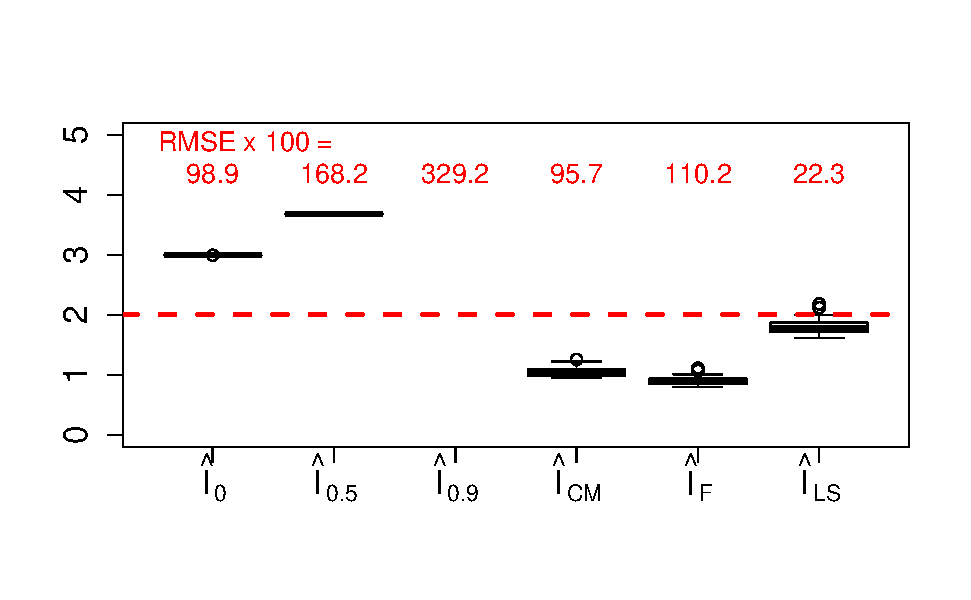
\includegraphics[scale = 0.6, clip = true, trim = 0 0.5in 0 0.5in]{../info_theory_sims/fig6.pdf}
\end{center}

\section{Discussion}

\subsubsection*{Acknowledgments}

Use unnumbered third level headings for the acknowledgments. All
acknowledgments go at the end of the paper. Do not include
acknowledgments in the anonymized submission, only in the final paper.

\section*{References}

References follow the acknowledgments. Use unnumbered first-level
heading for the references. Any choice of citation style is acceptable
as long as you are consistent. It is permissible to reduce the font
size to \verb+small+ (9 point) when listing the references. {\bf
  Remember that you can use a ninth page as long as it contains
  \emph{only} cited references.}
\medskip

\small

[X] Gastpar, M.  Gill, P.  Huth, A.  Theunissen, F. ``Anthropic Correction of Information Estimates and Its Application to Neural Coding.'' \emph{IEEE Trans. Info. Theory}, Vol 56 No 2, 2010.

[X] A. Borst and F. E. Theunissen, ``Information theory and neural coding''
Nature Neurosci., vol. 2, pp. 947?957, Nov. 1999.

[X] L. Paninski, ``Estimation of entropy and mutual information,'' Neural
Comput., vol. 15, no. 6, pp. 1191?1253, 2003.

[X] I. Nelken, G. Chechik, T. D. Mrsic-Flogel, A. J. King, and J. W. H.
Schnupp, ``Encoding stimulus information by spike numbers and mean
response time in primary auditory cortex,'' J. Comput. Neurosci., vol.
19, pp. 199?221, 2005.

[X] Cover and Thomas.  Elements of information theory.

[X]  Muirhead.  Aspects of multivariate statistical theory.

[X] van der Vaart.  Asymptotic statistics.

[1] Alexander, J.A.\ \& Mozer, M.C.\ (1995) Template-based algorithms
for connectionist rule extraction. In G.\ Tesauro, D.S.\ Touretzky and
T.K.\ Leen (eds.), {\it Advances in Neural Information Processing
  Systems 7}, pp.\ 609--616. Cambridge, MA: MIT Press.

[2] Bower, J.M.\ \& Beeman, D.\ (1995) {\it The Book of GENESIS:
  Exploring Realistic Neural Models with the GEneral NEural SImulation
  System.}  New York: TELOS/Springer--Verlag.

[3] Hasselmo, M.E., Schnell, E.\ \& Barkai, E.\ (1995) Dynamics of
learning and recall at excitatory recurrent synapses and cholinergic
modulation in rat hippocampal region CA3. {\it Journal of
  Neuroscience} {\bf 15}(7):5249-5262.

\end{document}
